\documentclass[
  aps,
  prd,
  preprint,
  nofootinbib,
  superscriptaddress,
  longbibliography
]{revtex4-2}

\usepackage{amsmath,amssymb,amsfonts}
\usepackage{bm}
\usepackage{array}
\usepackage{booktabs}
\usepackage{tikz}
\usepackage{placeins}
\usepackage[hidelinks]{hyperref}
\usetikzlibrary{arrows.meta,positioning,shapes.geometric}

\newcommand{\Spin}{\mathrm{Spin}}
\newcommand{\SO}{\mathrm{SO}}
\newcommand{\SU}{\mathrm{SU}}
\newcommand{\U}{\mathrm{U}}
\newcommand{\CP}{\mathbb{CP}}
\newcommand{\cO}{\mathcal{O}}
\newcommand{\GeV}{\mathrm{GeV}}
\DeclareMathOperator{\Tr}{Tr}
\DeclareMathOperator{\Res}{Res}

\newtheorem{theorem}{Theorem}[section]
\newtheorem{proposition}[theorem]{Proposition}
\newtheorem{lemma}[theorem]{Lemma}
\newtheorem{corollary}[theorem]{Corollary}
\newtheorem{definition}[theorem]{Definition}
\newtheorem{assumption}[theorem]{Assumption}
\newtheorem{datum}[theorem]{Benchmark Datum}
\newtheorem{observation}[theorem]{Observation}
\newtheorem{remark}[theorem]{Remark}
\newenvironment{proof}{\par\noindent\textit{Proof.}\ }{\hfill\(\square\)\par}

\begin{document}

\title{\texorpdfstring{A Face-Projection \(\Spin(10)\) Effective Framework:\\
Rubik Covariance, \(O(2)\) Family Geometry, and the Conditional GUT Boundary}
{A Face-Projection Spin(10) Effective Framework: Rubik Covariance, O(2) Family Geometry, and the Conditional GUT Boundary}}
\author{BoYu Chen}
\email{boypatrick.tw@gmail.com}
\affiliation{Independent Researcher, Hsinchu, Taiwan}
\date{May 22, 2026}

\begin{abstract}
This draft rewrites the theory around a face-projection principle.  Low-energy
Standard-Model labels are not treated as primitive entries in a table; they are
the projections of a higher-dimensional internal representation under a chosen
symmetry-breaking face.  In this language, one \(\Spin(10)\) half-spinor
\(16\) is the standard minimal six-face realization whose Standard-Model
projection displays
\[
  Q,\quad L,\quad u^c,\quad d^c,\quad \nu^c,\quad e^c .
\]
Three families are protected separately by the index
\[
  H^0(\CP^1,\cO(2)),\qquad \dim H^0(\CP^1,\cO(2))=3 .
\]
The result is not an unconditional PSLT-only derivation of a unique grand
unified theory.  It is a conditional \(\Spin(10)\) effective framework.  The
Majorana contact tensor direction is no longer left arbitrary: it is the unique
\(SL(2)\)-invariant second-transvectant direction \(K_{\rm tr}\).  An optional
Route-B hidden-messenger mechanism for \(\zeta K_{\rm tr}\) is recorded as a
conditional extension, but it is not part of the Route-A theorem core.  An
optional Route-D appendix records local string-constrained interpretations of
the same skeleton.  The hidden phase/radial sector and the companion audits
for flavor, proton decay, thresholds, and source-sector UV origin remain open.
Full phenomenological audits are deferred to companion work.
\end{abstract}

\maketitle

\section{Scope of the Lean Route-A Note}

This version is deliberately a Route-A paper skeleton.  Its theorem-level
claims are limited to three representation-geometric statements:
\[
\begin{array}{ll}
\text{six faces} & \Spin(10)\text{ half-spinor restriction gives one SM
family plus }\nu^c,\\
\text{three copies} & \Spin^c(\CP^1,\cO(2))\text{ Dolbeault index gives
three protected sections},\\
\text{contact direction} & K_{\rm tr}\text{ is the unique }SL(2)\text{
second-transvectant direction}.
\end{array}
\]
Route B is kept only as a conditional candidate mechanism for the complex
coefficient \(\zeta\).  Route D is kept only as a local string-constrained
interpretation of some of the same conditional data, not as a global
compactification.  Full CKM/PMNS fitting, dimension-five proton-decay Wilson
tensors, threshold matching, and source-sector UV completion are not claimed
in this lean note; they remain companion-audit problems.

\section{Face Projection}

The organizing idea is that the visible particle table is a projection table,
not a table of fundamental labels.  Let \(G\) be a high-energy compact group,
let \(R\) be a complex representation of \(G\), and let a vacuum orientation
\(\theta\) select a broken subgroup
\[
  H_\theta\simeq \SU(3)_C\times\SU(2)_L\times\U(1)_Y .
\]
The face projection is the restriction functor
\[
  \Pi_\theta(R):=\Res^{G}_{H_\theta}R
  =\bigoplus_\alpha m_{\alpha,\theta}\,r_{\alpha,\theta},
\]
where the irreducible \(H_\theta\)-summands \(r_{\alpha,\theta}\) are the
visible multiplet types.  If \(g\in G\), then the embedded subgroup changes by
conjugation,
\[
  H_\theta\longmapsto H_{g\theta}=gH_\theta g^{-1}.
\]
The same high-energy representation can therefore display different visible
labels under a different face:
\[
  \Pi_{g\theta}(R)
  =
  \Res^{G}_{gH_\theta g^{-1}}R .
\]
This is the representation-theoretic version of the intuitive statement that
the same internal object can look different after a legal internal rotation.

\begin{definition}[Rubik covariance]
A unified model is face-covariant if the visible low-energy multiplet types are
irreducible summands in restrictions of a common high-energy representation,
and if every allowed change of face is a conjugation of the broken-subgroup
embedding preserving anomaly cancellation, index, chirality, charge
normalization, and representation dimension.  The principle does not allow
arbitrary transmutation of low-energy particles.  It says that different
low-energy labels can be different visible faces of the same high-energy
object.
\end{definition}

The Rubik-cube image is useful only in this precise sense.  A chemical element
is still defined by nuclear charge; it does not become another element because
one rotates a drawing.  The analogy points instead to root lattices, Weyl
chambers, gauge-basis rotations, and symmetry-breaking projections.

The concrete grand-unification branch used below follows the standard
Pati--Salam and \(\Spin(10)\) route
\cite{PatiSalam1974,Georgi1975,FritzschMinkowski1975,Slansky1981}.  The conditional
neutrino sector uses the usual type-I seesaw logic
\cite{Minkowski1977,GellMannRamondSlansky1979,Yanagida1979}, while the
threshold language is the conventional perturbative RGE language
\cite{Jones1982,MachacekVaughn1983}.

\begin{figure*}[t]
\centering
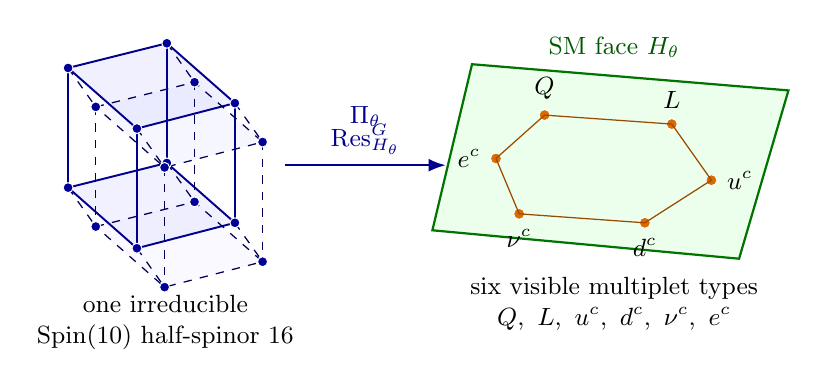
\begin{tikzpicture}[
  scale=0.95,
  every node/.style={font=\small},
  vertex/.style={circle, fill=blue!60!black, draw=white, line width=0.35pt,
    minimum size=3.6pt, inner sep=0pt},
  smpt/.style={circle, fill=orange!85!black, draw=white, line width=0.35pt,
    minimum size=4pt, inner sep=0pt},
  edge/.style={blue!55!black, line width=0.7pt},
  ghost/.style={blue!35!black, line width=0.45pt, dashed},
  proj/.style={-{Latex[length=2.2mm]}, thick, blue!55!black}
]
% A projected high-dimensional half-spin object.
\coordinate (a) at (-4.35,1.05);
\coordinate (b) at (-3.03,1.38);
\coordinate (c) at (-2.12,0.58);
\coordinate (d) at (-3.43,0.24);
\coordinate (e) at (-4.35,-0.55);
\coordinate (f) at (-3.03,-0.22);
\coordinate (g) at (-2.12,-1.02);
\coordinate (h) at (-3.43,-1.36);
\coordinate (aa) at (-3.98,0.53);
\coordinate (bb) at (-2.66,0.86);
\coordinate (cc) at (-1.75,0.06);
\coordinate (dd) at (-3.06,-0.28);
\coordinate (ee) at (-3.98,-1.07);
\coordinate (ff) at (-2.66,-0.74);
\coordinate (gg) at (-1.75,-1.54);
\coordinate (hh) at (-3.06,-1.88);
\fill[blue!15, opacity=0.40] (a)--(b)--(c)--(d)--cycle;
\fill[blue!20, opacity=0.28] (e)--(f)--(g)--(h)--cycle;
\fill[blue!12, opacity=0.28] (aa)--(bb)--(cc)--(dd)--cycle;
\fill[blue!10, opacity=0.22] (ee)--(ff)--(gg)--(hh)--cycle;
\draw[edge] (a)--(b)--(c)--(d)--cycle;
\draw[edge] (e)--(f)--(g)--(h)--cycle;
\draw[edge] (a)--(e) (b)--(f) (c)--(g) (d)--(h);
\draw[ghost] (aa)--(bb)--(cc)--(dd)--cycle;
\draw[ghost] (ee)--(ff)--(gg)--(hh)--cycle;
\draw[ghost] (aa)--(ee) (bb)--(ff) (cc)--(gg) (dd)--(hh);
\draw[ghost] (a)--(aa) (b)--(bb) (c)--(cc) (d)--(dd)
  (e)--(ee) (f)--(ff) (g)--(gg) (h)--(hh);
\foreach \p in {a,b,c,d,e,f,g,h,aa,bb,cc,dd,ee,ff,gg,hh}
  \node[vertex] at (\p) {};
\node[align=center] at (-3.05,-2.35)
  {one irreducible\\\(\Spin(10)\) half-spinor \(16\)};

% Projection arrow.
\draw[proj] (-1.45,-0.25) -- (0.70,-0.25)
  node[midway, above, align=center] {\(\Pi_\theta\)\\[-1mm]\(\Res^G_{H_\theta}\)};

% The Standard-Model face.
\coordinate (p1) at (1.05,1.10);
\coordinate (p2) at (5.28,0.75);
\coordinate (p3) at (4.62,-1.50);
\coordinate (p4) at (0.52,-1.12);
\fill[green!10, opacity=0.72] (p1)--(p2)--(p3)--(p4)--cycle;
\draw[green!45!black, line width=0.8pt] (p1)--(p2)--(p3)--(p4)--cycle;
\node[align=center, green!35!black] at (2.95,1.33)
  {SM face \(H_\theta\)};

\node[smpt, label=above:\(Q\)] at (2.02,0.42) {};
\node[smpt, label=above:\(L\)] at (3.72,0.30) {};
\node[smpt, label=right:\(u^c\)] at (4.25,-0.45) {};
\node[smpt, label=below:\(d^c\)] at (3.36,-1.02) {};
\node[smpt, label=below:\(\nu^c\)] at (1.68,-0.90) {};
\node[smpt, label=left:\(e^c\)] at (1.37,-0.16) {};
\draw[orange!60!black, line width=0.45pt]
  (2.02,0.42)--(3.72,0.30)--(4.25,-0.45)--(3.36,-1.02)
  --(1.68,-0.90)--(1.37,-0.16)--cycle;
\node[align=center] at (2.95,-2.10)
  {six visible multiplet types\\
  \(Q,\ L,\ u^c,\ d^c,\ \nu^c,\ e^c\)};
\end{tikzpicture}
\caption{Face-projection geometry.  The \(16\) is visualized as a single
higher-dimensional internal object whose Standard-Model face displays the six
visible multiplet types \(Q,L,u^c,d^c,\nu^c,e^c\).  The figure is a
representation-geometric visualization, not a dynamical particle-conversion
process.}
\label{fig:face-projection}
\end{figure*}

\section{\texorpdfstring{The Six-Face \(\Spin(10)\) Object}{The Six-Face Spin(10) Object}}

\begin{proposition}[Standard minimal six-face realization]
Among standard simple compact GUT candidates, if the six chiral
Standard-Model multiplet types
\[
  Q,\quad L,\quad u^c,\quad d^c,\quad \nu^c,\quad e^c
\]
are required to arise from one irreducible complex chiral representation whose
restriction contains exactly one SM family plus \(\nu^c\), with no chiral SM
exotics and with minimal representation dimension, the standard minimal
single-object realization is the \(\Spin(10)\) half-spinor \(16\).
\end{proposition}

\begin{proof}
The Pati--Salam subgroup of \(\Spin(10)\) gives
\[
  16\to (4,2,1)\oplus(\bar 4,1,2).
\]
Breaking
\[
  \SU(4)_C\to \SU(3)_C\times \U(1)_{B-L}
\]
gives
\[
  4\to (3,1/3)\oplus(1,-1),\qquad
  \bar4\to(\bar3,-1/3)\oplus(1,+1).
\]
With
\[
  Y=T_{3R}+\frac{B-L}{2},
\]
the restriction to the Standard-Model face is
\[
  \Res^{\Spin(10)}_{G_{\rm SM}}16
  =
  Q\oplus L\oplus u^c\oplus d^c\oplus\nu^c\oplus e^c,
\]
where the six projected Standard-Model multiplet types are
\[
\begin{array}{c|c}
\text{field} & \SU(3)_C\times\SU(2)_L\times\U(1)_Y\\
\hline
Q & (3,2)_{1/6}\\
L & (1,2)_{-1/2}\\
u^c & (\bar3,1)_{-2/3}\\
d^c & (\bar3,1)_{1/3}\\
\nu^c & (1,1)_0\\
e^c & (1,1)_1 .
\end{array}
\]
The \(SU(5)\) alternative uses \(10\oplus\bar5\oplus1\), which is not one
irreducible chiral object.  Pati--Salam is natural but not simple.  \(E_6\)
contains this structure inside a larger \(27\), usually bringing extra matter
that must be lifted.  Therefore \(\Spin(10)\) with a \(16\) is the standard
minimal single-object realization.
\end{proof}

\begin{proposition}[Hypercharge normalization]
The face projection
\[
  Y=T_{3R}+\frac{B-L}{2}
\]
has the GUT normalization
\[
  \frac{\Tr Y^2}{\Tr T_{3L}^2}=\frac53 .
\]
\end{proposition}

\begin{proof}
The trace is over one left-handed \(16\) after Standard-Model decomposition.
For one family,
\[
\Tr Y^2=
6\left(\frac16\right)^2
+2\left(-\frac12\right)^2
+3\left(-\frac23\right)^2
+3\left(\frac13\right)^2
+1(1)^2
+1(0)^2
=\frac{10}{3}.
\]
The \(SU(2)_L\) doublets are \(Q\) and \(L\), and the doublet normalization is
\(\Tr_{\bf 2}T_3^2=1/2\).  Hence
\[
  \Tr T_{3L}^2=3\cdot\frac12+1\cdot\frac12=2.
\]
Thus
\[
  \frac{\Tr Y^2}{\Tr T_{3L}^2}=\frac{10/3}{2}=\frac53.
\]
\end{proof}

\begin{remark}[Allowed meaning of rotation]
At low energy \(Q\) cannot be freely rotated into \(e^c\).  The Standard-Model
gauge symmetry has already selected fixed visible labels.  The face-projection
statement is about the high-energy representation and its broken-subgroup
projection.  Any physical process that changes the visible face must be
mediated by legitimate high-energy fields and is constrained, for example, by
proton decay.
\end{remark}

\section{\texorpdfstring{Three Families from an \(O(2)\) Index}{Three Families from an O(2) Index}}

The family number is not produced by rotating the six-face object.  It is a
separate index statement.  The analytic input is the standard
\(\Spin^c\) Dolbeault--Dirac/cohomology identification and the
Riemann--Roch--Serre-duality calculation on \(\CP^1\)
\cite{LawsonMichelsohn1989,GriffithsHarris1978}.

\begin{figure*}[t]
\centering
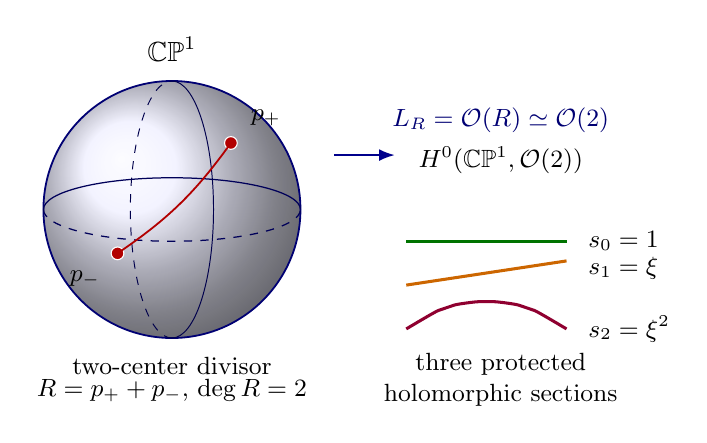
\begin{tikzpicture}[
  scale=0.96,
  every node/.style={font=\small},
  marked/.style={circle, fill=red!70!black, draw=white, line width=0.4pt,
    minimum size=4.6pt, inner sep=0pt},
  section/.style={line width=1.1pt, rounded corners=3pt}
]
% Riemann sphere with two divisor points.
\shade[ball color=blue!7, opacity=0.92] (0,0) circle (1.7);
\draw[blue!45!black, line width=0.65pt] (0,0) circle (1.7);
\draw[blue!35!black, line width=0.45pt] (-1.7,0) arc[start angle=180,end angle=0,
  x radius=1.7, y radius=0.42];
\draw[blue!35!black, dashed, line width=0.45pt] (-1.7,0)
  arc[start angle=180,end angle=360, x radius=1.7, y radius=0.42];
\draw[blue!30!black, line width=0.35pt] (0,-1.7) arc[start angle=-90,end angle=90,
  x radius=0.55, y radius=1.7];
\draw[blue!30!black, dashed, line width=0.35pt] (0,-1.7)
  arc[start angle=-90,end angle=-270, x radius=0.55, y radius=1.7];
\node[font=\normalsize] at (0,2.12) {\(\CP^1\)};
\node[marked, label={[xshift=2pt,yshift=1pt]above right:\(p_+\)}] at (0.78,0.88) {};
\node[marked, label={[xshift=-1pt,yshift=-1pt]below left:\(p_-\)}] at (-0.72,-0.58) {};
\draw[red!70!black, line width=0.65pt] (0.78,0.88) to[bend left=10] (-0.72,-0.58);
\node[align=center] at (0,-2.25) {two-center divisor\\[-1mm]
  \(R=p_+ + p_-\), \(\deg R=2\)};

% Bundle label and protected sections.
\draw[-{Latex[length=2mm]}, thick, blue!55!black] (2.15,0.72) -- (2.95,0.72);
\node[align=center, blue!45!black] at (4.35,1.18)
  {\(L_R=\cO(R)\simeq\cO(2)\)};
\node[align=center] at (4.35,0.65)
  {\(H^0(\CP^1,\cO(2))\)};

% Three section profiles, drawn as geometric modes rather than boxes.
\draw[section, green!45!black] (3.10,-0.42) -- (5.22,-0.42);
\draw[section, orange!80!black] (3.10,-1.00) -- (5.22,-0.68);
\draw[section, purple!75!black]
  plot[smooth] coordinates {(3.10,-1.58) (3.63,-1.30) (4.16,-1.22)
  (4.69,-1.30) (5.22,-1.58)};
\node[right] at (5.38,-0.42) {\(s_0=1\)};
\node[right] at (5.38,-0.78) {\(s_1=\xi\)};
\node[right] at (5.38,-1.58) {\(s_2=\xi^2\)};
\node[align=center] at (4.35,-2.25) {three protected\\holomorphic sections};
\end{tikzpicture}
\caption{Two-center geometry of the family carrier.  The two marked points
define a degree-two divisor \(R=p_++p_-\), hence the line bundle
\(L_R\simeq\cO(2)\).  The family count comes from the protected section space
\(H^0(\CP^1,\cO(2))=\mathrm{span}\{1,\xi,\xi^2\}\), not from treating the
two centers as two families.  This is a topology/complex-geometry picture, not
a dynamical flow diagram.}
\label{fig:two-center-o2}
\end{figure*}

Figure~\ref{fig:two-center-o2} is the geometric picture behind the theorem:
the two centers set the degree of the line bundle, while Riemann--Roch and
Serre duality fix the number of protected sections.

\begin{theorem}[Conditional \(\Spin^c\) index theorem for three protected families]
Assume that the protected internal family carrier is the \(\Spin^c\)
Dolbeault bundle on
\[
  C=\CP^1
\]
twisted by a two-center divisor
\[
  R=p_+ + p_-,
  \qquad
  L_R=\cO(R)\simeq \cO(2).
\]
Assume also that all other SM-charged internal sectors are absent, gapped, or
vectorlike, so they contribute no additional unpaired chiral zero modes.  Let
\[
  D_R=\sqrt2\left(\bar\partial_{L_R}+\bar\partial_{L_R}^\dagger\right)
\]
be the corresponding \(\Spin^c\) Dolbeault--Dirac operator.  Then
\[
  \ker D_R^+\simeq H^0(\CP^1,\cO(2)),\qquad
  \ker D_R^-\simeq H^1(\CP^1,\cO(2)),
\]
with
\[
  \dim H^0(\CP^1,\cO(2))=3,
\]
and \(H^1(\CP^1,\cO(2))=0\).  Thus the protected sector contributes exactly
three positive-chirality family zero modes.
\end{theorem}

\begin{proof}
Hodge theory identifies the positive and negative \(\Spin^c\)
Dolbeault--Dirac kernels with the Dolbeault cohomology groups displayed above.
Riemann--Roch on \(\CP^1\) gives
\[
  h^0(\CP^1,\cO(2))-h^1(\CP^1,\cO(2))=2+1=3.
\]
Serre duality gives
\[
  h^1(\CP^1,\cO(2))
  =h^0(\CP^1,K_{\CP^1}\otimes\cO(-2))
  =h^0(\CP^1,\cO(-4))=0.
\]
Therefore \(h^0=3\).
\end{proof}

\begin{corollary}[Projected chiral state space]
Under the six-face \(\Spin(10)\) assumption and the \(O(2)\) family carrier,
the low-energy chiral state space is
\[
  {\cal S}_{\rm chiral}^{4D}
  =
  16\otimes H^0(\CP^1,\cO(2))
  \simeq
  16_1\oplus16_2\oplus16_3 .
\]
\end{corollary}

\begin{remark}[Why this is still conditional]
This theorem does not derive \(C=\CP^1\), the two-center divisor \(R\), the
\(\Spin^c\) carrier, or the no-extra-unpaired-sector condition.
Those are branch assumptions.  The theorem says that once those inputs are
chosen, the family count is protected and is not a tunable scan output.
\end{remark}

\begin{remark}[Tangent-bundle reading of the same carrier]
On the rational family curve,
\[
  T_{\CP^1}\simeq \cO(2),
  \qquad
  H^0(\CP^1,T_{\CP^1})\simeq \mathfrak{sl}_2(\mathbb C).
\]
Thus, after the branch choice \(L_R\simeq\cO(2)\), the protected three-section
space can also be read as the holomorphic vector-field algebra of the
rational curve.  This does not derive the curve \(C=\CP^1\) or the divisor
input; it only shows that the \(\cO(2)\) carrier, the three protected modes,
and the \(SL(2)\) family covariance are three views of the same rational-curve
geometry.  In an affine coordinate \(\xi\), the vector field
\(\xi\partial_\xi\) vanishes at \(0\) and \(\infty\); in this reading the two
marked points \(p_\pm\) can be viewed as a Cartan choice on the rational
curve, up to \(PGL(2)\) conjugation.
\end{remark}

\begin{remark}[Genus cap for the tangent reading]
The tangent-bundle reading is special to the rational curve.  For a compact
Riemann surface \(\Sigma_g\),
\[
  h^0(\Sigma_g,T_{\Sigma_g})
  =
  \begin{cases}
  3,& g=0,\\
  1,& g=1,\\
  0,& g\ge2.
  \end{cases}
\]
Indeed, \(T_{\Sigma_g}\simeq K_{\Sigma_g}^{-1}\) has degree \(2-2g\); for
\(g=0\) it is \(\cO(2)\), for \(g=1\) it is trivial, and for \(g\ge2\) it has
negative degree.  Thus, within this tangent interpretation, three protected
holomorphic vector fields are the rational-curve maximum, not a generic curve
feature.
\end{remark}

\FloatBarrier

\section{Conditional EFT Data}

The face-projection and index principles supply the representational skeleton.
They do not by themselves determine the full action.  The current conditional
branch retains the following action-level data:
\[
\begin{array}{ll}
{\rm A1} & \Spin(10)\text{ face-projection EFT with complete }16_i,\\
{\rm A2} & H^0(\CP^1,\cO(2))\text{ protects three copies of the }16,\\
{\rm A3} & \text{type-I seesaw with a source-fixed Majorana contact},\\
{\rm A4} & \text{proton bounds and two-loop threshold matching},\\
{\rm A5} & \text{constrained/composite }54/210\text{ source order parameters},\\
{\rm A6} & \text{auxiliary/composite conormal multipliers},\\
{\rm A7} & \text{a Schur lock with singlet auxiliaries and sterile completion}.
\end{array}
\]

\begin{figure}[!htbp]
\centering
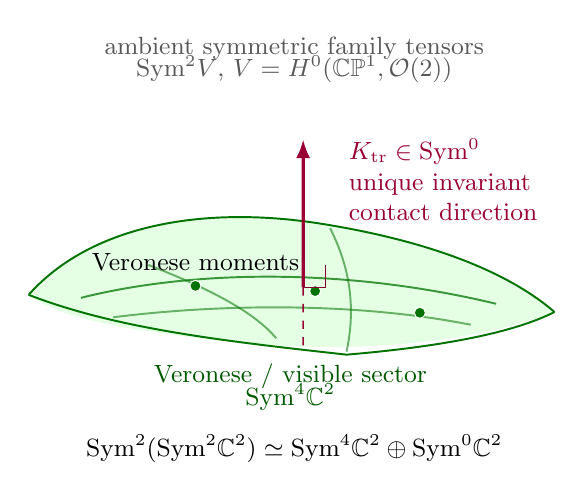
\begin{tikzpicture}[
  scale=0.95,
  every node/.style={font=\small},
  surface/.style={green!45!black, line width=0.7pt},
  contact/.style={-{Latex[length=2.4mm]}, purple!80!black, line width=1.2pt},
  moment/.style={circle, fill=green!45!black, draw=white, line width=0.35pt,
    minimum size=4pt, inner sep=0pt}
]
% Ambient symmetric tensor space.
\node[align=center, gray!70!black] at (0,2.42)
  {ambient symmetric family tensors\\[-1mm]
  \(\mathrm{Sym}^2V\), \(V=H^0(\CP^1,\cO(2))\)};

% Veronese/moment sector as a curved sheet.
\fill[green!12, opacity=0.86]
  (-3.55,-0.72) .. controls (-2.75,0.18) and (-1.30,0.48) .. (0.30,0.24)
  .. controls (1.72,0.02) and (2.82,-0.38) .. (3.48,-0.95)
  .. controls (2.36,-1.38) and (0.70,-1.52) .. (-0.92,-1.34)
  .. controls (-2.36,-1.18) and (-3.14,-1.02) .. (-3.55,-0.72);
\draw[surface]
  (-3.55,-0.72) .. controls (-2.75,0.18) and (-1.30,0.48) .. (0.30,0.24)
  .. controls (1.72,0.02) and (2.82,-0.38) .. (3.48,-0.95);
\draw[surface]
  (-3.55,-0.72) .. controls (-2.36,-1.18) and (-0.92,-1.34) .. (0.70,-1.52)
  .. controls (2.36,-1.38) and (3.10,-1.14) .. (3.48,-0.95);
\draw[surface, opacity=0.75]
  (-2.85,-0.76) .. controls (-1.42,-0.40) and (0.62,-0.34) .. (2.70,-0.84);
\draw[surface, opacity=0.55]
  (-2.42,-1.02) .. controls (-0.82,-0.82) and (0.95,-0.84) .. (2.36,-1.12);
\draw[surface, opacity=0.55]
  (-1.95,-0.32) .. controls (-0.92,-0.72) and (-0.48,-1.02) .. (-0.24,-1.30);
\draw[surface, opacity=0.55]
  (0.48,0.17) .. controls (0.76,-0.38) and (0.82,-0.92) .. (0.70,-1.48);

\node[moment, label=above:\(\text{Veronese moments}\)] at (-1.32,-0.60) {};
\node[moment] at (0.28,-0.67) {};
\node[moment] at (1.68,-0.96) {};
\node[align=center, green!35!black] at (-0.05,-1.95)
  {Veronese / visible sector\\[-1mm]\(\mathrm{Sym}^4\mathbb C^2\)};

% Unique transverse singlet contact direction.
\coordinate (base) at (0.12,-0.62);
\draw[purple!80!black, dashed, line width=0.55pt] (base) -- (0.12,-1.40);
\draw[contact] (base) -- (0.12,1.36);
\node[purple!80!black, align=left, anchor=west] at (0.60,0.82)
  {\(K_{\rm tr}\in\mathrm{Sym}^0\)\\unique invariant\\contact direction};
\draw[purple!70!black, line width=0.6pt] (0.12,-0.62) -- (0.42,-0.62) -- (0.42,-0.32);

% Decomposition statement.
\node[align=center] at (0,-2.78)
  {\(\mathrm{Sym}^2(\mathrm{Sym}^2\mathbb C^2)
  \simeq
  \mathrm{Sym}^4\mathbb C^2\oplus\mathrm{Sym}^0\mathbb C^2\)};
\end{tikzpicture}
\caption{Veronese sector and contact direction.  The curved sheet visualizes
the \(\mathrm{Sym}^4\mathbb C^2\) Veronese/moment sector inside
\(\mathrm{Sym}^2V\), while the transverse direction is the unique scalar
summand \(K_{\rm tr}\in\mathrm{Sym}^0\).  The contact tensor is therefore not
an arbitrary patch; it is the unique invariant direction outside the visible
Veronese sector.}
\label{fig:veronese-contact}
\end{figure}

\FloatBarrier

Figure~\ref{fig:veronese-contact} summarizes the representation-theoretic
split used in the next lemma: the tensor direction of the Majorana contact is
fixed, while its complex coefficient is separate conditional data.

\begin{lemma}[Unique \(SL(2)\)-invariant contact direction]
\label{lem:ktr-contact}
Let
\[
  V=H^0(\CP^1,\cO(2))\simeq \mathrm{Sym}^2\mathbb C^2.
\]
Then
\[
  \mathrm{Sym}^2 V
  \simeq
  \mathrm{Sym}^4\mathbb C^2\oplus \mathrm{Sym}^0\mathbb C^2.
\]
The Veronese moment sector is the \(\mathrm{Sym}^4\mathbb C^2\) summand,
while the orthogonal singlet contact sector is unique up to phase.  In the
normalized \((\psi_0,\psi_1,\psi_2)\) basis used for the family carrier, this
singlet can be represented as
\[
  K_{\rm tr}
  =
  \frac1{\sqrt3}
  \begin{pmatrix}
    0&0&-1\\
    0&1&0\\
    -1&0&0
  \end{pmatrix}.
\]
Coordinate-free, \(K_{\rm tr}\in \mathrm{Sym}^2V^\vee\) and its inverse
bilinear form is \(K_{\rm tr}^{-1}\in \mathrm{Sym}^2V\).  In the displayed
orthonormal basis, the induced matrix obeys
\[
  K_{\rm tr}^2=\frac13 I,\qquad K_{\rm tr}^{-1}=3K_{\rm tr}.
\]
\end{lemma}

\begin{proof}
This is the Clebsch--Gordan decomposition for
\(\mathrm{Sym}^2(\mathrm{Sym}^2\mathbb C^2)\)
\cite{FultonHarris1991}.  The scalar summand has
multiplicity one, so any invariant symmetric contact tensor is proportional to
the displayed second-transvectant matrix.
\end{proof}

\begin{remark}[Killing-form reading]
Using the tangent-bundle identification
\[
  V=H^0(\CP^1,\cO(2))\simeq H^0(\CP^1,T_{\CP^1})
  \simeq \mathfrak{sl}_2(\mathbb C),
\]
the same invariant line can be read as the Killing-form line on the
automorphism algebra of the rational family curve.  The displayed
\(K_{\rm tr}\) differs from the conventional Killing matrix only by the chosen
\(SU(2)\)-orthonormal basis, sign, and overall normalization.  This gives the
contact direction a geometric pairing interpretation, but it still does not
turn \(SL(2)\) into a fundamental global symmetry.
\end{remark}

\begin{remark}[Meaning of the \(SL(2)\) covariance]
The \(SL(2)\) language in Lemma~\ref{lem:ktr-contact} is used as
family-geometry covariance, or equivalently as spurionic bookkeeping for the
rational curve.  It is not claimed to be an exact fundamental global symmetry.
Any microscopic or quantum-gravity completion must realize this covariance
geometrically, locally, or through spurions rather than as an unbroken global
selection rule.  Appendix~\ref{app:route-d-string} records one local
string-constrained interpretation of this kind of geometric realization.
\end{remark}

\begin{datum}[Majorana contact]
The benchmark Majorana matrix is not purely Veronese.  It requires the unique
orthogonal second-transvectant contact component
\[
  \frac{M_R}{M_*}=M_V+\zeta K_{\rm tr},
\]
with
\[
  \zeta=0.1076472949+0.0736514853\,i.
\]
The contact fraction is
\[
  \frac{\|\zeta K_{\rm tr}\|}{\|M_R/M_*\|}
  =1.304275\times10^{-1}.
\]
\end{datum}

The companion machine audit that produced the previous long draft decomposes
the inverse-seesaw reconstructed \(M_R\)
into the Veronese subspace plus the orthogonal trace/contact direction.  The
Veronese-plus-contact residual is at machine precision, whereas the
Veronese-only residual equals the displayed contact fraction.  This means the
contact is not a negligible correction to the present PMNS-compatible branch.
The lean note records the datum and the geometrically fixed tensor direction;
the full matrices, basis cards, and norm conventions are deferred to companion
artifacts.

\begin{observation}[Hidden-origin scan]
Tested simple hidden-quotient and small monomial clockwork classes do not
derive \(\zeta\).  In those classes, it remains a conditional datum.
\end{observation}

The scan evidence is limited but sharp within that tested class.  The
contact-sensitivity scan gives the loose PMNS-compatible windows
\[
  \Delta s=3.208798\times10^{-5},\qquad
  \Delta\delta=5.424119\times10^{-5}\ {\rm rad}.
\]
Removing the contact spoils the PMNS and mass-splitting replay.  A minimal
hidden \(D\)-quotient leaves modulus and phase flat directions.  A small
real-coefficient monomial or clockwork phase with denominator \(N\le6\) misses
the target phase by at least
\[
  4.471595\times10^{-1}\ {\rm rad},
\]
and the first root of unity inside the loose phase window appears only at
\[
  N=178.
\]
Thus no small hidden quotient or small monomial clockwork mechanism in the
current evidence set predicts the complex value of \(\zeta\).  A future
non-minimal hidden sector may still do so, but it would be a new assumption
that must be audited with its threshold and UV cost.

\section{\texorpdfstring{Optional Route B: Hidden Transvectant Origin for \(\zeta\)}{Optional Route B: Hidden Transvectant Origin for zeta}}

The negative scan above does not forbid a hidden origin for \(\zeta\).  It only
says that the currently tested small hidden quotients and small monomial
clockwork classes do not predict it.  This section is an optional conditional
extension, not part of the Route-A theorem core.  The conservative Route-B move is
therefore to add a new hidden-sector theorem: derive the tensor direction from
the unique transvectant \(K_{\rm tr}\), and isolate the remaining burden in a
hidden phase/radial sector that supplies the complex number.

\begin{theorem}[Post-\(B-L\) sterile transvectant messenger]
Let
\[
  V=H^0(\CP^1,\cO(2)).
\]
After \(B-L\) breaking, let
\[
  N_i=P_{\nu^c}(16_i),\qquad N\in V,
\]
be the right-handed neutrino family vector selected by the Majorana source
projector.  Let
\[
  X\in V^\vee
\]
be a visible-singlet sterile family messenger.  At the post-\(B-L\) matching
scale, consider the coordinate-free superpotential
\[
  \frac{W_R}{M_*}
  =
  \frac12 M_V(N,N)
  +\lambda X(N)
  -\frac12 K_{\rm tr}^{-1}(X,X),
\]
where
\[
  M_V\in\mathrm{Sym}^2V^\vee,\qquad
  K_{\rm tr}\in\mathrm{Sym}^2V^\vee,\qquad
  K_{\rm tr}^{-1}\in\mathrm{Sym}^2V.
\]
In a chosen basis this is
\[
  \frac{W_R}{M_*}
  =
  \frac12 N^T M_V N
  +\lambda X^T N
  -\frac12 X^T K_{\rm tr}^{-1}X,
\]
where \(K_{\rm tr}\) is the unique \(SL(2)\)-invariant contact direction from
Lemma~\ref{lem:ktr-contact}.  Integrating out \(X\) gives
\[
  \frac{W_R^{\rm eff}}{M_*}
  =
  \frac12\left(M_V+\lambda^2K_{\rm tr}\right)(N,N).
\]
Thus the benchmark contact is generated if
\[
  \lambda^2=\zeta.
\]
\end{theorem}

\begin{proof}
The \(X\)-F-term is the equality in \(V\)
\[
  \frac{\partial W_R}{\partial X}
  =
  M_*\left(\lambda N-K_{\rm tr}^{-1}X\right)=0.
\]
Here \(K_{\rm tr}^{-1}:V^\vee\to V\) is the inverse map induced by the
non-degenerate bilinear form \(K_{\rm tr}\).  Thus
\[
  X=\lambda K_{\rm tr}N,
\]
where \(K_{\rm tr}:V\to V^\vee\).  Substitution gives, in any basis,
\[
\begin{aligned}
  \frac{W_R^{\rm eff}}{M_*}
  &=
  \frac12 M_V(N,N)
  +\lambda X(N)
  -\frac12 K_{\rm tr}^{-1}(X,X)\\
  &=
  \frac12 M_V(N,N)
  +\lambda^2K_{\rm tr}(N,N)
  -\frac12\lambda^2K_{\rm tr}(N,N)\\
  &=
  \frac12\left(M_V+\lambda^2K_{\rm tr}\right)(N,N).
\end{aligned}
\]
Equivalently, in matrix notation,
\[
  \frac{W_R^{\rm eff}}{M_*}
  =
  \frac12 N^T M_V N+\frac12\lambda^2N^TK_{\rm tr}N .
\]
This is exactly the displayed effective Majorana matrix.
\end{proof}

\begin{remark}[Scope of the projector]
The field \(N_i=P_{\nu^c}(16_i)\) is a post-\(B-L\)-breaking EFT variable.
Before symmetry breaking, a \(\Spin(10)\)-singlet messenger cannot select
\(\nu^c\) from the \(16_i\) without an additional Majorana source or
projector.  Route B therefore assumes such a post-breaking projector, for
example from a \((B-L)=-2\) Majorana source sector, rather than deriving it
from face projection alone.  In this lean note \(P_{\nu^c}\) is therefore an
input of the post-\(B-L\) EFT matching problem, not a result of the
face-projection principle.  In conventional \(\SO(10)\) language, one
possible source of this post-breaking projection is a \(\overline{126}_H\)
Majorana source: its Pati--Salam \((10,1,3)\) component contains an
SM-singlet direction that pairs with the \(\nu^c\nu^c\) bilinear.  This is
only a source-sector interpretation here, not a completed UV model.
\end{remark}

\begin{datum}[Target coefficient]
For the current benchmark,
\[
  \zeta_{\rm tar}=0.1076472949+0.0736514853\,i.
\]
Its polar data are
\[
  \begin{aligned}
  |\zeta_{\rm tar}|&=0.13043190325293763,\\
  \arg\zeta_{\rm tar}&=0.600038020318215 .
  \end{aligned}
\]
One square-root coupling is
\[
  \lambda=\sqrt{\zeta_{\rm tar}}
  =
  0.34502115743308964
  +0.10673473744038917\,i,
\]
with
\[
  |\lambda|=0.3611535729477664.
\]
This is a moderate hidden coupling; it is not a high-power clockwork
suppression.
\end{datum}

\begin{remark}[Printed precision versus physical precision]
The many digits in \(\zeta_{\rm tar}\), \(|\zeta_{\rm tar}|\), and
\(\lambda\) are kept as reproducibility anchors for the benchmark files.  They
should not be read as ten-digit physical predictions.  The optional
instanton interpretation in Appendix~\ref{app:route-d-string} already has
expected higher-order corrections of order \(|\zeta|^2\simeq1.7\times10^{-2}\),
and the finite-messenger canonical-normalization estimate below gives
\(|\lambda|^2/(16\pi^2)\simeq8.26\times10^{-4}\).  Until the companion
flavor/proton/threshold audits are replayed in a concrete UV completion, only
the first few significant figures should be treated as physically meaningful.
\end{remark}

\begin{observation}[\(\mathbb Z_{178}\) phase diagnostic]
A discrete phase can approximate the benchmark phase by
\[
  \zeta_{178}
  =
  |\zeta_{\rm tar}|\exp\left(\frac{2\pi i\,17}{178}\right).
\]
Since
\[
  \frac{2\pi\,17}{178}=0.6000794956295111,
\]
the phase error is
\[
  4.1475311296\times10^{-5}\ {\rm rad},
\]
which lies inside the loose phase window
\[
  5.424119\times10^{-5}\ {\rm rad}.
\]
The direct complex error is
\[
  |\zeta_{178}-\zeta_{\rm tar}|
  =
  5.4097037899\times10^{-6}.
\]
This does not make \(\zeta\) an exact prediction.  It supplies a precise
discrete-phase candidate; exact equality would require either a small axion
shift or a continuous hidden phase.  The Route-B hidden-messenger theorem uses
only \(\lambda^2=\zeta\); the \(\mathbb Z_{178}\) value is kept as a side
diagnostic, not as a premise of the benchmark branch.  Diophantine
approximations of this kind are generic for any real phase.  For
\(\arg\zeta/(2\pi)=0.09549901697671904\), the continued-fraction convergents
include
\[
  \frac{17}{178},\qquad \frac{70}{733},\qquad \frac{87}{911},
\]
with phase errors
\[
  4.15\times10^{-5},\qquad 6.68\times10^{-6},\qquad
  2.73\times10^{-6}\ {\rm rad}.
\]
Thus if the admissible phase window is tightened below the \(178\)-denominator
error, the diagnostic must move to higher-denominator approximants.  The
stringy axion-volume option in Appendix~\ref{app:route-d-string} is the more
physical way to interpret a continuous hidden phase.
\end{observation}

\begin{observation}[Nonperturbative hidden-spurion option]
An alternative is
\[
  \zeta=Ae^{-S_H+i\theta_H}.
\]
For \(A=1\),
\[
  S_H=-\log|\zeta_{\rm tar}|=2.0369040025655094,\qquad
  \theta_H=\arg\zeta_{\rm tar}.
\]
This is naturally interpreted as a nonperturbative hidden-sector spurion.  It
is a conditional physical origin, not a weak-coupling derivation from
face-projection alone.  Appendix~\ref{app:route-d-string} records the local
E3-instanton/Green--Schwarz version of this interpretation.
\end{observation}

\begin{lemma}[Minimal post-\(B-L\) \(R\)-selection rule]
\label{lem:routeb-r-selection}
At the post-\(B-L\) matching scale, take the superpotential to have
\(R(W)=2\).  A minimal selection rule that keeps the sterile messenger
Majorana-only is
\[
\begin{array}{c|c|c}
\text{object} & \text{role} & U(1)_R\\
\hline
16_i\text{ components} & \text{matter multiplets, including }N_i & 1\\
H,T,\bar T & \text{Higgs doublet/triplet fields} & 0\\
X\in V^\vee & \text{sterile transvectant messenger} & 1\\
\lambda,\ M_V,\ K_{\rm tr}^{-1} & \text{matching tensors/spurions} & 0
\end{array}
\]
together with the post-breaking projector
\[
  N_i=P_{\nu^c}(16_i).
\]
Then the Route-B Majorana terms
\[
  X(N),\qquad K_{\rm tr}^{-1}(X,X),\qquad M_V(N,N)
\]
all have \(R=2\), while ordinary Dirac and triplet Yukawa terms
\[
  16_i16_jH,\qquad 16_i16_jT
\]
also have \(R=2\).  However any superpotential operator with at least one
additional \(X\) inserted into a Dirac or colored-triplet operator has
\[
  R=2+m,\qquad m\ge1,
\]
and is therefore forbidden if the \(R\)-selection rule is exact at the
matching scale.
\end{lemma}

\begin{proof}
The allowed Route-B terms have
\[
  R(X)+R(N)=1+1=2,\qquad
  2R(X)=2,\qquad
  2R(N)=2.
\]
The baseline Dirac and triplet Yukawa terms have
\[
  R(16_i)+R(16_j)+R(H\text{ or }T)=1+1+0=2.
\]
Adding \(m\ge1\) sterile messengers to such an operator shifts the
superpotential charge to \(2+m\), so the operator is not allowed.  This proves
the selection rule at the holomorphic matching level.  If later \(R\)-breaking
spurions are introduced, they must be charged so that these forbidden
operators remain absent to the order being audited.
\end{proof}

\begin{remark}[Status of the \(R\)-selection rule]
The \(U(1)_R\) assignment in Lemma~\ref{lem:routeb-r-selection} is used here as
a holomorphic EFT matching selection rule.  It is not yet claimed to be an
anomaly-free microscopic symmetry.  A UV implementation would require either
an anomaly-free continuous or discrete \(R\)-symmetry, or a spurionic origin
whose \(R\)-breaking insertions do not regenerate \(X\)-decorated Dirac or
colored-triplet operators within the audited order.  Appendix~\ref{app:route-d-string}
gives a local Green--Schwarz/Stueckelberg interpretation of the same kind of
selection-rule bookkeeping, again without claiming a global compactification.
\end{remark}

\begin{theorem}[Tree-level matching silence]
In a canonical-normalized post-\(B-L\) EFT at the matching scale, use Route B
as a post-\(B-L\)-breaking matching theorem, with
\[
  N_i=P_{\nu^c}(16_i)
\]
as above.  Assume the hidden messenger sector obeys the \(R\)-selection rule of
Lemma~\ref{lem:routeb-r-selection}:
\[
  X\ \text{is a visible singlet},\qquad
  X\ \text{couples only to the Majorana channel }K_{\rm tr}(N,N),
\]
and \(X\) has no couplings to Dirac Yukawa operators or colored-triplet
operators.  If integrating out \(X\) gives
\[
  \Delta M_R/M_*=\zeta K_{\rm tr},
\]
then the visible one-loop threshold vector, the Dirac Yukawa matrices, and the
dimension-five colored-triplet Wilson tensors are unchanged relative to the
benchmark.
\end{theorem}

\begin{proof}
Since \(X\) is a visible singlet,
\[
  \Delta b_1^X=\Delta b_2^X=\Delta b_3^X=0,
\]
so it contributes no non-universal visible one-loop threshold.  The
Majorana-only selection rule gives
\[
  \delta Y_u=\delta Y_d=\delta Y_e=\delta Y_{\nu D}=0.
\]
The same rule forbids hidden insertions in the colored-triplet Yukawa
couplings and inverse triplet propagator, so
\[
  \delta C_{5L}=\delta C_{5R}=0.
\]
If \(\zeta\) equals the benchmark value, then \(M_R\) is the benchmark
Majorana matrix and the type-I seesaw replay is unchanged.  Thus the hidden
contact can generate the missing Majorana tensor without moving the visible
flavor, proton-decay, or one-loop threshold audits.
\end{proof}

\begin{observation}[Canonical basis caveat]
The theorem above holds at tree level after canonical normalization.  A
microscopic completion with a finite messenger interval can generate a
right-handed-neutrino wave-function correction of order
\[
  \delta Z_N\sim
  \frac{|\lambda|^2}{16\pi^2}
  \log\frac{M_*}{M_X}.
\]
For the benchmark value,
\[
  \frac{|\lambda|^2}{16\pi^2}
  =
  8.259697\times10^{-4}.
\]
This is small, but not automatically smaller than the narrow
contact-sensitivity windows.  Therefore the benchmark matrices in this lean
note are defined after canonical normalization.  If a microscopic model
predicts a non-negligible \(\delta Z_N\), the companion seesaw replay must use
\[
  Y_{\nu D}\mapsto Y_{\nu D}\left(1-\frac12\delta Z_N\right),
\]
\[
  M_R\mapsto
  M_R-\frac12\left(\delta Z_N^T M_R+M_R\delta Z_N\right),
\]
before comparing to the PMNS benchmark.
\end{observation}

The compact numerical checks for this optional Route-B extension are recorded
separately in Appendix~\ref{app:routeb-checks}; they are algebraic matching
checks, not companion phenomenology audits.

\section{Theorem Boundary}

\begin{theorem}[Conditional benchmark boundary]
Given the face-projection data, the \(O(2)\) index data, the companion
benchmark audits, and either a benchmark-specified Majorana datum
\(\mathcal D_\zeta\) or a Route-B hidden messenger producing
\(\mathcal D_{\rm hidden\ zeta}\), the current construction defines one
internally checked conditional EFT branch:
\[
\begin{array}{c}
\mathcal D_{\rm face}
\, +\, \mathcal D_{\rm index}
\, +\, (\mathcal D_{\zeta}\ \text{or}\ \mathcal D_{\rm hidden\ zeta})
\, +\, \mathcal D_{\mathrm{companion\ audits}}\\
\hline
\leadsto\ \text{one conditional benchmark branch}.
\end{array}
\]
This does not support the stronger implication
\[
  \text{PSLT/Another Physics alone}
  \Longrightarrow
  \text{a unique GUT with predicted }\zeta .
\]
\end{theorem}

\begin{proof}
A complete microscopic GUT requires an explicit gauge group, chiral matter
representations, anomaly cancellation, a breaking potential, Yukawa and
Majorana sectors, baryon-violating operators, and threshold matching.
Face projection motivates the \(\Spin(10)\) representation geometry.
The \(O(2)\) index protects the family count.  Neither supplies all
action-level data.  The remaining branch data A1--A7 and the benchmark-level
checks are conditional inputs or companion artifacts, and they are required
whether \(\zeta\) is supplied as a benchmark datum or generated through Route
B.  The Route-B messenger derives \(\zeta K_{\rm tr}\) only after adding a
hidden sterile messenger, phase/radial data, and Majorana-only selection
rules.  It therefore improves the conditional EFT explanation of \(\zeta\),
but it is still not a PSLT-only prediction and it does not replace the
companion phenomenological audits.
\end{proof}

\begin{corollary}[Status of the rewritten theory]
The complete claim of this lean version is
\[
\boxed{
\begin{gathered}
\text{face-projection motivation}
+\text{ conditional }\Spin(10)\text{ EFT}\\
\neq
\text{unconditional PSLT-only GUT proof}.
\end{gathered}
}
\]
The rewrite is nevertheless useful: it gives a coherent representation-level
reason why \(\Spin(10)\) is the natural minimal six-face family object and why
three families are protected by an independent \(O(2)\) index.
\end{corollary}

\section{Minimal Reproducibility Manifest}

The lean note has a small, explicit reproducibility surface.  It does not
include the deferred full flavor/proton/threshold scans.
\begin{itemize}
\item Paper source: \texttt{paper/gut\_framework.tex} and
\texttt{paper/refs.bib}.
\item Compiled note: \texttt{paper/gut\_framework.pdf}.
\item D5 appendix check:
\texttt{python3 code/verify\_d5\_half\_spin\_hypercube.py}.
\item D5 outputs: summary, weights, and report in
\texttt{output/d5\_half\_spin/}.
\item Optional Route-B algebra check:
\texttt{python3 code/verify\_hidden\_zeta\_origin.py}.
\item Optional Route-B output: verification JSON in
\texttt{output/hidden\_zeta\_origin/}\\
\texttt{routeB\_hidden\_zeta\_verification.json}.
\item Optional Route-D local string checks:
\texttt{python3 route\_d/code/}\\
\texttt{verify\_d1\_f\_theory\_local\_placement.py}
and\\
\texttt{python3 route\_d/code/}\\
\texttt{verify\_d2\_e3\_instanton\_zeta.py}.
\item Optional Route-D outputs:
\texttt{route\_d/output/d1\_f\_theory\_local\_placement.*} and
\texttt{route\_d/output/d2\_e3\_instanton\_zeta.*}.
\item Deferred-audit convention card:
\path{code/audit0_conventions_card.py}, with local output
\path{output/audit0/invariant_card.*}.
\item Deferred-audit scaffolds:
\path{code/audit1_flavor_target_conventions.py} and\\
\path{code/audit4a_source_spectrum_schema.py}, with local outputs in\\
\path{output/audit1/} and \path{output/audit4a/}.
\item Status log: \texttt{roadmap.md}.
\end{itemize}
The reproducible numerical claims inside this TeX draft are therefore only the
D5 half-spin branching check, the hypercharge normalization check, the
Route-B algebraic \(\zeta K_{\rm tr}\) matching check, and the appendix-level
Route-D local string-placement/instanton arithmetic.  The Audit 0/1/4a files
are convention and schema cards for future work, not phenomenology results.
All publication-grade phenomenology remains outside this manifest until the
companion audits are restored.

\section{Deferred Calculations}

Earlier drafts contained detailed scan and audit material for Yukawa textures,
\(d=5\) proton decay, threshold corrections, source sectors, clockwork rescue,
and theorem ledgers.  Those artifacts are preserved in the project history,
but they are omitted from this lean TeX draft because their status relative to
the face-projection principle is not yet settled.  The only numerical Route-B
checks kept here are the algebraic \(\zeta\), \(K_{\rm tr}\), and
phase-spurion checks needed for the optional hidden messenger theorem.

The paper strategy is therefore:
\[
\begin{array}{ll}
\text{Route A} &
\text{main paper: representation/index/contact skeleton},\\
\text{Route B} &
\text{optional extension or companion: hidden origin for }\zeta,\\
\text{Route D} &
\text{optional appendix: local string-constrained interpretation},\\
\text{companion audits} &
\text{full flavor, }d=5\text{ proton decay, thresholds, source-sector UV}.
\end{array}
\]
The companion-audit dependency graph is fixed in the generated Audit 0 card as
\[
  0 \longrightarrow (1\parallel 4a)\longrightarrow 3\longrightarrow 2,
\]
with \(4b\) as an optional Route-D/global-geometry track.  Audit 1 currently
fixes only the flavor/seesaw target-table contract and marks publication
targets as requiring refresh.  Audit 4a currently fixes only the source-sector
heavy-spectrum schema and records that no non-placeholder
\texttt{heavy\_spectrum.json} has yet been exported.  Thus Audit 3 remains
blocked on a source spectrum, and Audit 2 remains blocked on both physical
flavor rotations and triplet inverse data.

\section{Lean-Note Status Ledger}

The logical status of this version is deliberately narrower than a complete
GUT construction:
\begin{description}
\item[Proved/constructed.]
\(\Spin(10)\) face skeleton; \(\Spin^c(\CP^1,\cO(2))\) index;
\(K_{\rm tr}\) uniqueness; optional Route-B Schur complement.
\item[Conditional inputs.]
\(C=\CP^1\), \(R=p_++p_-\); protected \(\Spin^c\) carrier;
no unpaired SM-charged exotics; \(P_{\nu^c}\); \(R\)-selection rule;
hidden phase/radial sector.
\item[Deferred audits.]
Full flavor fit; \(d=5\) proton-decay Wilson tensors;
threshold/proton companion audits; source-sector UV origin.
\item[Optional UV interpretations.]
Route-D local F-theory placement and E3-instanton interpretation of
\(\zeta K_{\rm tr}\), both with global compactification and zero-mode caveats.
\item[Not claimed.]
PSLT-only unique GUT proof.
\end{description}

\section{Conclusion}

The clean result of the rewrite is a bounded theorem stack.  A \(\Spin(10)\)
half-spinor supplies a standard minimal six-face object; the
\(\Spin^c(\CP^1,\cO(2))\) carrier supplies three protected copies; and the
second-transvectant singlet supplies the unique Majorana contact direction.
These are mathematical inputs and consequences inside a conditional EFT
branch.  They do not by themselves determine the microscopic source sector,
the complex hidden coefficient \(\zeta\), the full flavor fit, or the
proton-decay Wilson tensors.  The optional Route-D appendix gives local
string-constrained interpretations of some conditional inputs, not a global
string compactification.  Keeping this boundary explicit is the point of the
lean Route-A version.  This note establishes the
representation/index/contact skeleton; it does not claim full GUT
phenomenology.

\appendix
\section{\texorpdfstring{\(D_5\) Half-Spin Weight Hypercube}{D5 Half-Spin Weight Hypercube}}

This appendix records the compact representation-theoretic calculation behind
the six-face statement.  It is not a new uniqueness theorem; it is the
weight-level explanation of the standard \(\Spin(10)\) half-spinor branch used
in the main text \cite{Slansky1981,FultonHarris1991}.

Let \(e_1,\ldots,e_5\) be an orthonormal basis for the \(D_5\) weight space.
The roots of \(D_5\) are
\[
  \pm e_a\pm e_b,\qquad a\ne b.
\]
Choose the positive-chirality half-spin representation to have weights
\[
  \Lambda_{16}
  =
  \left\{
  \frac12\sum_{a=1}^5 s_a e_a:
  s_a=\pm1,\quad
  \#\{a:s_a=-1\}\equiv0\pmod2
  \right\}.
\]
There are \(2^{5-1}=16\) such weights.  The Pati--Salam face is the split
\[
  D_5\supset D_3\oplus D_2,
  \qquad
  \Spin(6)\times\Spin(4)
  \simeq
  \SU(4)_C\times\SU(2)_L\times\SU(2)_R.
\]
Use \(s_1,s_2,s_3\) for the \(D_3\) spinor weights and \(s_4,s_5\) for the
\(D_2\) spinor weights.  Define
\[
  m_C=\#\{a\le3:s_a=-1\},\qquad
  m_W=\#\{a=4,5:s_a=-1\}.
\]
The chirality condition says \(m_C+m_W\) is even, so \(m_C\) and \(m_W\) have
the same parity.  Therefore the weights split into exactly two blocks:
\[
\begin{array}{c|c|c|c}
m_C\ {\rm parity} & m_W\ {\rm parity} & \text{number of weights}
& \text{Pati--Salam block}\\
\hline
{\rm even} & {\rm even} & 4\cdot2=8 & (4,2,1)\\
{\rm odd} & {\rm odd} & 4\cdot2=8 & (\bar4,1,2).
\end{array}
\]
Thus
\[
  16\to (4,2,1)\oplus(\bar4,1,2).
\]

One convenient convention for the \(\SU(4)_C\) component is
\[
\begin{array}{c|c|c}
\text{first three signs} & \SU(3)_C & B-L\\
\hline
\text{zero minus signs} & 1 & -1\\
\text{two minus signs} & 3 & 1/3\\
\text{one minus sign} & \bar3 & -1/3\\
\text{three minus signs} & 1 & 1 .
\end{array}
\]
For the weak \(D_2\) signs, take
\[
  (s_4,s_5)=(+,+),(-,-)
  \quad\Longrightarrow\quad
  \SU(2)_L\text{ doublet},\quad
  T_{3L}=\frac{s_4+s_5}{4},\quad T_{3R}=0,
\]
and
\[
  (s_4,s_5)=(+,-),(-,+)
  \quad\Longrightarrow\quad
  \SU(2)_R\text{ doublet},\quad
  T_{3R}=\frac{s_4-s_5}{4},\quad T_{3L}=0.
\]
Applying
\[
  Y=T_{3R}+\frac{B-L}{2}
\]
then gives the six visible Standard-Model faces:
\[
\begin{array}{c|c|c|c}
\text{field} & \SU(3)_C\times\SU(2)_L & Y & \text{multiplicity}\\
\hline
Q & (3,2) & 1/6 & 6\\
L & (1,2) & -1/2 & 2\\
u^c & (\bar3,1) & -2/3 & 3\\
d^c & (\bar3,1) & 1/3 & 3\\
\nu^c & (1,1) & 0 & 1\\
e^c & (1,1) & 1 & 1 .
\end{array}
\]
The multiplicities sum to \(16\), so this is a complete half-spinor, not a
collection of separately chosen low-energy fragments.

\begin{figure*}[t]
\centering
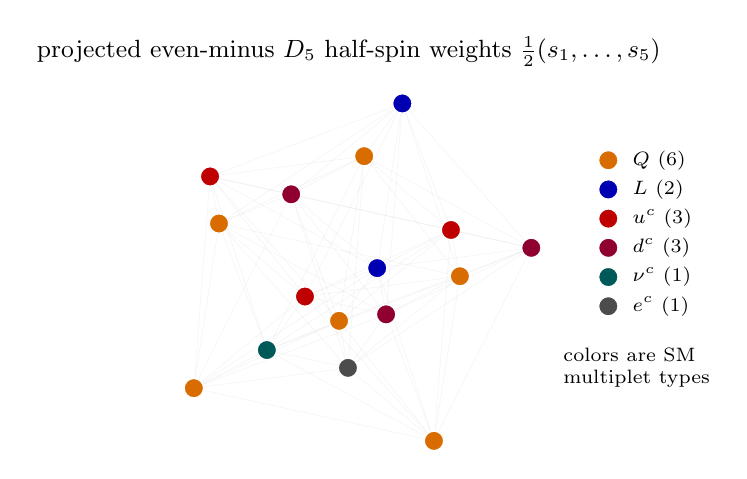
\begin{tikzpicture}[
  scale=1.03,
  every node/.style={font=\small},
  spinEdge/.style={gray!45, opacity=0.16, line width=0.28pt},
  weight/.style={circle, draw=white, line width=0.45pt, minimum size=7pt,
    inner sep=0pt},
  weightQ/.style={weight, fill=orange!85!black},
  weightL/.style={weight, fill=blue!70!black},
  weightU/.style={weight, fill=red!75!black},
  weightD/.style={weight, fill=purple!75!black},
  weightNu/.style={weight, fill=teal!70!black},
  weightE/.style={weight, fill=black!70},
  legendText/.style={anchor=west, font=\scriptsize}
]
\node[align=center] at (0,2.72)
  {projected even-minus \(D_5\) half-spin weights
  \(\frac12(s_1,\ldots,s_5)\)};

\coordinate (w0) at (0.35,0.05); % +++++ L
\coordinate (w1) at (0.66,2.08); % +++-- L
\coordinate (w2) at (2.25,0.30); % ++-+- d^c
\coordinate (w3) at (1.26,0.52); % ++--+ u^c
\coordinate (w4) at (0.46,-0.52); % +-++- d^c
\coordinate (w5) at (-0.54,-0.30); % +-+-+ u^c
\coordinate (w6) at (1.05,-2.08); % +--++ Q
\coordinate (w7) at (1.37,-0.05); % +---- Q
\coordinate (w8) at (-0.71,0.96); % -+++- d^c
\coordinate (w9) at (-1.71,1.18); % -++-+ u^c
\coordinate (w10) at (-0.12,-0.60); % -+-++ Q
\coordinate (w11) at (0.19,1.43); % -+--- Q
\coordinate (w12) at (-1.91,-1.43); % --+++ Q
\coordinate (w13) at (-1.60,0.60); % --+-- Q
\coordinate (w14) at (-0.01,-1.18); % ---+- e^c
\coordinate (w15) at (-1.01,-0.96); % ----+ nu^c

% Demihypercube edges: pairs of even-parity sign words differing in two signs.
\draw[spinEdge] (w0) -- (w1);
\draw[spinEdge] (w0) -- (w2);
\draw[spinEdge] (w0) -- (w3);
\draw[spinEdge] (w0) -- (w4);
\draw[spinEdge] (w0) -- (w5);
\draw[spinEdge] (w0) -- (w6);
\draw[spinEdge] (w0) -- (w8);
\draw[spinEdge] (w0) -- (w9);
\draw[spinEdge] (w0) -- (w10);
\draw[spinEdge] (w0) -- (w12);
\draw[spinEdge] (w1) -- (w2);
\draw[spinEdge] (w1) -- (w3);
\draw[spinEdge] (w1) -- (w4);
\draw[spinEdge] (w1) -- (w5);
\draw[spinEdge] (w1) -- (w7);
\draw[spinEdge] (w1) -- (w8);
\draw[spinEdge] (w1) -- (w9);
\draw[spinEdge] (w1) -- (w11);
\draw[spinEdge] (w1) -- (w13);
\draw[spinEdge] (w2) -- (w3);
\draw[spinEdge] (w2) -- (w4);
\draw[spinEdge] (w2) -- (w6);
\draw[spinEdge] (w2) -- (w7);
\draw[spinEdge] (w2) -- (w8);
\draw[spinEdge] (w2) -- (w10);
\draw[spinEdge] (w2) -- (w11);
\draw[spinEdge] (w2) -- (w14);
\draw[spinEdge] (w3) -- (w5);
\draw[spinEdge] (w3) -- (w6);
\draw[spinEdge] (w3) -- (w7);
\draw[spinEdge] (w3) -- (w9);
\draw[spinEdge] (w3) -- (w10);
\draw[spinEdge] (w3) -- (w11);
\draw[spinEdge] (w3) -- (w15);
\draw[spinEdge] (w4) -- (w5);
\draw[spinEdge] (w4) -- (w6);
\draw[spinEdge] (w4) -- (w7);
\draw[spinEdge] (w4) -- (w8);
\draw[spinEdge] (w4) -- (w12);
\draw[spinEdge] (w4) -- (w13);
\draw[spinEdge] (w4) -- (w14);
\draw[spinEdge] (w5) -- (w6);
\draw[spinEdge] (w5) -- (w7);
\draw[spinEdge] (w5) -- (w9);
\draw[spinEdge] (w5) -- (w12);
\draw[spinEdge] (w5) -- (w13);
\draw[spinEdge] (w5) -- (w15);
\draw[spinEdge] (w6) -- (w7);
\draw[spinEdge] (w6) -- (w10);
\draw[spinEdge] (w6) -- (w12);
\draw[spinEdge] (w6) -- (w14);
\draw[spinEdge] (w6) -- (w15);
\draw[spinEdge] (w7) -- (w11);
\draw[spinEdge] (w7) -- (w13);
\draw[spinEdge] (w7) -- (w14);
\draw[spinEdge] (w7) -- (w15);
\draw[spinEdge] (w8) -- (w9);
\draw[spinEdge] (w8) -- (w10);
\draw[spinEdge] (w8) -- (w11);
\draw[spinEdge] (w8) -- (w12);
\draw[spinEdge] (w8) -- (w13);
\draw[spinEdge] (w8) -- (w14);
\draw[spinEdge] (w9) -- (w10);
\draw[spinEdge] (w9) -- (w11);
\draw[spinEdge] (w9) -- (w12);
\draw[spinEdge] (w9) -- (w13);
\draw[spinEdge] (w9) -- (w15);
\draw[spinEdge] (w10) -- (w11);
\draw[spinEdge] (w10) -- (w12);
\draw[spinEdge] (w10) -- (w14);
\draw[spinEdge] (w10) -- (w15);
\draw[spinEdge] (w11) -- (w13);
\draw[spinEdge] (w11) -- (w14);
\draw[spinEdge] (w11) -- (w15);
\draw[spinEdge] (w12) -- (w13);
\draw[spinEdge] (w12) -- (w14);
\draw[spinEdge] (w12) -- (w15);
\draw[spinEdge] (w13) -- (w14);
\draw[spinEdge] (w13) -- (w15);
\draw[spinEdge] (w14) -- (w15);

\node[weightL] at (w0) {};
\node[weightL] at (w1) {};
\node[weightD] at (w2) {};
\node[weightU] at (w3) {};
\node[weightD] at (w4) {};
\node[weightU] at (w5) {};
\node[weightQ] at (w6) {};
\node[weightQ] at (w7) {};
\node[weightD] at (w8) {};
\node[weightU] at (w9) {};
\node[weightQ] at (w10) {};
\node[weightQ] at (w11) {};
\node[weightQ] at (w12) {};
\node[weightQ] at (w13) {};
\node[weightE] at (w14) {};
\node[weightNu] at (w15) {};

% Color legend.
\node[weightQ] at (3.20,1.38) {};
\node[legendText] at (3.38,1.38) {\(Q\) \((6)\)};
\node[weightL] at (3.20,1.02) {};
\node[legendText] at (3.38,1.02) {\(L\) \((2)\)};
\node[weightU] at (3.20,0.66) {};
\node[legendText] at (3.38,0.66) {\(u^c\) \((3)\)};
\node[weightD] at (3.20,0.30) {};
\node[legendText] at (3.38,0.30) {\(d^c\) \((3)\)};
\node[weightNu] at (3.20,-0.06) {};
\node[legendText] at (3.38,-0.06) {\(\nu^c\) \((1)\)};
\node[weightE] at (3.20,-0.42) {};
\node[legendText] at (3.38,-0.42) {\(e^c\) \((1)\)};
\node[align=left, font=\scriptsize] at (3.55,-1.18)
  {colors are SM\\multiplet types};
\end{tikzpicture}
\caption{Projected \(D_5\) half-spin weight hypercube.  The \(16\) even-parity
half-spin weights are shown as one projected demihypercube and colored by
their Standard-Model multiplet type after the Pati--Salam face projection.
The multiplicities reproduce
\((Q,L,u^c,d^c,\nu^c,e^c)=(6,2,3,3,1,1)\).}
\label{fig:d5-half-spin-hypercube}
\end{figure*}

The appendix calculation is reproduced by
\[
  \texttt{code/verify\_d5\_half\_spin\_hypercube.py}.
\]
The generated summary reports
\[
  \#\Lambda_{16}=16,\qquad
  (4,2,1):8,\qquad
  (\bar4,1,2):8,
\]
the six field multiplicities
\[
  (Q,L,u^c,d^c,\nu^c,e^c)=(6,2,3,3,1,1),
\]
and the same normalization check as in the main text,
\[
  \Tr Y^2=\frac{10}{3},\qquad
  \Tr T_{3L}^2=2,\qquad
  k_Y=\frac53.
\]

\section{Optional Route-D String-Constrained Placement}
\label{app:route-d-string}

This appendix records the promotion decision for Route D.  The local
F-theory placement audit and the E3-instanton audit are included only as a
string-constrained interpretation of the Route-A/Route-B data.  They are not
part of the Route-A theorem core and do not constitute a global F-theory
compactification.

\subsection{Local \texorpdfstring{\(D_5\to E_6\)}{D5 to E6} placement}

In local F-theory GUT models, a gauge algebra is engineered on a divisor by
the singular fiber type.  A \(D_5\) singularity realizes
\(\mathfrak{so}(10)\), while charged matter can localize on curves where the
singularity enhances in codimension two.  The Katz--Vafa local rule identifies
the matter from the adjoint branching of the enhanced algebra
\cite{KatzVafa1996,BeasleyHeckmanVafa2008I}.  For a \(D_5\to E_6\)
enhancement,
\[
  E_6\supset \SO(10)\times\U(1),
\]
and
\[
  \mathbf{78}
  =
  \mathbf{45}_0
  \oplus
  \mathbf{1}_0
  \oplus
  \mathbf{16}_{-3}
  \oplus
  \overline{\mathbf{16}}_{+3}.
\]
The dimension check is
\[
  45+1+16+16=78.
\]
Thus the six-face \(\Spin(10)\) object used in the main text has a standard
local string interpretation: the \(\mathbf{16}\) appears as one irreducible
matter curve representation, rather than as six separately chosen
Standard-Model fragments.

The same local picture can reproduce the \(O(2)\) family carrier.  On a
matter curve \(\Sigma=\CP^1\), the zero-mode carrier is represented as
\[
  K_\Sigma^{1/2}\otimes L_{\rm flux}.
\]
Since
\[
  K_{\CP^1}^{1/2}=\cO(-1),
\]
a flux bundle with degree three gives
\[
  K_{\CP^1}^{1/2}\otimes \cO(3)
  =
  \cO(-1)\otimes\cO(3)
  =
  \cO(2).
\]
Consequently
\[
  h^0(\CP^1,\cO(2))=3,\qquad
  h^1(\CP^1,\cO(2))=0.
\]
This does not eliminate conditional input; it replaces the abstract
\(\cO(2)\) assumption by the flux-quantized matter-curve datum
\[
  2=3_{\rm flux}-1_{\rm spin}.
\]

\begin{remark}[Global caveat]
The local \(D_5\to E_6\) branching and the \(\CP^1\) index do not verify a
global F-theory compactification.  Hypercharge flux or Wilson-line breaking
must still satisfy the global massless-hypercharge condition and avoid chiral
exotics and uncontrolled threshold corrections
\cite{BeasleyHeckmanVafa2008II,MayrhoferPaltiWeigand2013}.
\end{remark}

\subsection{E3-instanton interpretation of \texorpdfstring{\(\zeta K_{\rm tr}\)}{zeta Ktr}}

The optional Route-B hidden messenger isolates the complex coefficient
\(\zeta\) from the tensor direction \(K_{\rm tr}\).  A standard Type IIB/F
theory interpretation of this coefficient is an Euclidean D3-brane instanton
factor
\cite{Witten1996,BlumenhagenCveticWeigand2006,IbanezUranga2006,CveticRichterWeigand2007}
\[
  \zeta_\Gamma=A_\Gamma e^{2\pi iT_\Gamma},
  \qquad
  T_\Gamma=\theta_\Gamma+i\,t_\Gamma.
\]
Thus the hidden phase/radial sector becomes an axion-volume pair.  For the
benchmark value
\[
  \zeta_{\rm tar}=0.1076472949+0.0736514853\,i,
\]
one has
\[
  |\zeta_{\rm tar}|=0.13043190325293763,
  \qquad
  \arg\zeta_{\rm tar}=0.600038020318215.
\]
For unit prefactor modulus,
\[
  S_{\rm eff}=-\log|\zeta_{\rm tar}|
  =
  2.0369040025655094,
\]
or, in the convention \(\zeta=\exp(2\pi iT_\Gamma)\),
\[
  \operatorname{Im}T_\Gamma=0.3241833406119675.
\]

The Majorana-only selection rule also has a standard instanton interpretation.
Perturbative abelian symmetries can survive as selection rules even when the
corresponding gauge bosons become massive by a Green--Schwarz/Stueckelberg
mechanism.  An instanton factor can transform under such a symmetry because
its axion shifts.  In a minimal charge ledger,
\[
  q(N)=+1,\qquad q(NN)=+2,\qquad q(e^{-S_\Gamma+i\varphi_\Gamma})=-2,
\]
so the instanton-dressed Majorana insertion is neutral:
\[
  q\!\left(e^{-S_\Gamma+i\varphi_\Gamma}NN\right)=0.
\]
In an actual compactification this bookkeeping must be realized by universal
and charged instanton zero modes, whose saturation pattern inserts \(N_iN_j\)
and does not generate the forbidden Dirac or colored-triplet operators
\cite{BianchiCollinucciMartucci2011,CveticDonagiHalversonMarsano2012}.

Finally, landing specifically on \(K_{\rm tr}\) requires the same locality or
equivariance assumption used in the Route-B discussion.  If the instanton data
are blind to detailed family coordinates on
\[
  V=H^0(\CP^1,\cO(2))\simeq \mathrm{Sym}^2\mathbb C^2
\]
except through the contact pairing, then the unique invariant contact
direction is the scalar second-transvectant summand
\[
  K_{\rm tr}\in\mathrm{Sym}^0
  \subset
  \mathrm{Sym}^2(\mathrm{Sym}^2\mathbb C^2)
  =
  \mathrm{Sym}^4\mathbb C^2\oplus\mathrm{Sym}^0.
\]

\begin{remark}[Precision caveat]
The instanton interpretation explains the form, selection rule, and moderate
scale of \(\zeta\).  It does not predict the benchmark value to many digits.
For the benchmark,
\[
  |\zeta|^2=0.01701248138618368,
\]
which is about
\[
  \frac{|\zeta|^2}{3.208798\times10^{-5}}
  =
  530.1823731560442
\]
times the recorded contact-sensitivity window.  Multi-instanton, multi-cover,
prefactor, and moduli-stabilization effects therefore cannot be ignored in any
claim of high-precision prediction.
\end{remark}

The appendix-level checks are reproduced by
\[
  \texttt{route\_d/code/verify\_d1\_f\_theory\_local\_placement.py}
\]
and
\[
  \texttt{route\_d/code/verify\_d2\_e3\_instanton\_zeta.py}.
\]

\section{\texorpdfstring{Optional Route-B Algebraic Checks}{Optional Route-B Algebraic Checks}}
\label{app:routeb-checks}

This table checks only the optional Route-B Schur-complement algebra.  It is
not a substitute for the deferred full flavor, proton-decay, threshold, or
source-sector audits.

\begin{table*}[t]
\centering
\small
\renewcommand{\arraystretch}{1.15}
\begin{tabular}{lll}
\toprule
\textbf{check} & \textbf{value} & \textbf{role}\\
\midrule
\(|\zeta_{\rm tar}|\) &
\(0.13043190325293763\) &
target modulus\\
\(\arg\zeta_{\rm tar}\) &
\(0.600038020318215\) &
target phase\\
\(\sqrt{\zeta_{\rm tar}}\) &
\(0.345021+0.106735\,i\) &
hidden messenger coupling\\
\(|\lambda|\) &
\(0.3611535729477664\) &
moderate coupling\\
\(\|\lambda^2K_{\rm tr}-\zeta K_{\rm tr}\|_F\) &
\(1.20185\times10^{-17}\) &
Schur-complement match\\
\(\|K_{\rm tr}(3K_{\rm tr})-I\|_F\) &
\(3.84593\times10^{-16}\) &
inverse convention\\
\(2\pi(17/178)-\arg\zeta\) &
\(4.14753\times10^{-5}\ {\rm rad}\) &
side phase diagnostic\\
\(|\zeta_{178}-\zeta_{\rm tar}|\) &
\(5.40970\times10^{-6}\) &
discrete approximation\\
\(-\log|\zeta|\) &
\(2.0369040025655094\) &
instanton-spurion option\\
\(|\lambda|^2/(16\pi^2)\) &
\(8.25970\times10^{-4}\) &
canonical-basis audit scale\\
\(\Delta b_{\rm vis}^{X}\) &
\((0,0,0)\) &
visible threshold silence\\
\bottomrule
\end{tabular}
\caption{Optional Route-B algebraic verification.}
\label{tab:routeb-zeta-checks}
\end{table*}

\bibliographystyle{apsrev4-2}
\bibliography{refs}

\end{document}
